\section{1174074 | Mochamad Arifqi Ramadhan}
\subsection{Teori}
\begin{enumerate}
	\item Definisi Sejarah dan Perkembangan Kecerdasan Buatan
	\hfill\break
	 Kecerdasan Buatan biasa disebut dengan istilah AI (Artificial Intelligence). AI sendiri merupakan suatu cabang dalam bisnis sains komputer sains dimana mengkaji tentang bagaimana cara untuk menlengkapi sebuah komputer dengan kemampuan atau kepintaran layaknya atau mirip dengan yang dimiliki manusia. Sebagai contoh, sebagaimana komputer dapat berkomunikasi dengan pengguna baik menggunakan kata, suara maupun lain sebagainya. Dengan kemampuan ini, diharapkan komputer mampu mengambil keputusan sendiri untuk berbagai kasus yang ditemuinya kemudian itulah yang disebut dengan kecerdasan buatan. Kecerdasan buatan adalah kemampuan komputer digital atau robot yang dikendalikan konputer untuk melakukan tugas yang umumnya dikaitkan dengan sesuatu yang cerdas. Istilah ini sering diterapkan pada proyek pengembangan sistem yang diberkahi dengan karakteristik proses intelektual manusia, seperti kemampuan untuk berpikir, menemukan makna, menggeneralisasi, atau belajar dari pengalaman masa lalu.

    Kecerdasan Buatan adalah salah satu bidang studi yang berhubungan dengan pemanfaatan mesin untuk memecahkan persoalan yang rumit dengan cara lebih manusiawi dan lebih bisa di pahami oleh manusia. Kecerdasan buatan makin canggih dengan kemampuan komputer dalam memperbarui pengetahuannya dengan banyaknya testing dan perkembangan target analisa. Untuk kecerdasan buatan ada banyak contoh dan jenisnya. Salah satu contoh yang paling terkenal dari Artificial Intelligence ialah Google Assistant. Google Assistant digunakan untuk kemudahan user dalam menemukan berbagai hal maupun penyetingan langsung terhadap smartphone yang digunakan dan masih banyak lagi.

	\hfill\break
	Sejarah Kecerdasan Buatan,  Artificial intelligence merupakan inovasi baru di bidang ilmu pengetahuan. Mulai terbentuk sejak adanya komputer modern dan kira-kira terjadi sekitaran tahun 1940 dan 1950. Ilmu pengetahuan komputer ini khusus ditujukan dalam perancangan otomatisasi tingkah laku cerdas dalam sistem kecerdasan komputer. Pada awal 50-an, studi tentang “mesin berpikir” memiliki berbagai nama seperti cybernetics, teori automata, dan pemrosesan innformasi. Pada tahun 1956, para ilmuan jenius seperti Alan Turing, Norbert, Wiener, Claude Shannon dan Warren McCullough telah bekerja secara independen dibidang cybernetics, matematika, algoritma dan teori jaringan. Namun, seprang ilmuan komputer dan kognitif John McCarthy adalah orang yang dating dengan ide untuk bergabung dengan upaya penelitian terpisah ini kedalam satu bidang yang akan mempelajari topic baru untuk imajinasi manusia yaitu kecerdasan buatan. Dia adalah orang yang menciptakan istilah tersebut dan kemudian mendirikan laboratorium Kecerdasan Buatan di MIT dan Stan ford.


    \hfill\break
    Perkembangan Kecerdasan Buatan, Teknologi Artificial Intelligence semakin ramai dibahas dalam berbagai diskusi teknologi di seluruh dunia.Menurut kebanyakan orang, pekerjaan seperti kasir, operator telepon, pengendara truk, dan lainnya sangat berpeluang besar untuk tergantikan oleh Artificial Intelligence. Mengapa terjadi hal demikian? dikarenakan memang bahwa AI lebih ungul dalam hal kinerja, fitur dan lain sebagainya. Namun, dalam beberapa aspek memang pekerja manusia masih unggul dibandingkan AI itu sendiri. Para generasi muda yang ada di dunia terutama di daerah Asia terlihat sudah memahami fungsi dan efek dari AI dalam kehidupan kita sehari-hari. Berdasarkan survei yang dilakukan oleh Microsoft, terdapat 39 persen responden yang mempertimbangkan untuk menggunakan mobil tanpa pengemudi dan 36 persen lainnya setuju bahwa robot masa depan dengan software untuk beroperasi mampu meningkatkan produktivitas. Dari survey tersebut kita sebagai pengguna AI harus lebih bijaksana dalam pengembangan dan penggunaan dari AI sehingga tanpa memberikan efek samping terhadap etos kerja dan keseharian kita sebagai pengguna dalam kehidupan sehari-hari.

   
	\item Definisi Supervised learning, klasifikasi, regresi, unsupervised learning, dataset, training set dan testing set.
	\hfill\break
	\begin{itemize}
		\item Supervised Learning
		\hfill\break
		Supervised Learning merupakan tugas pengumpulan data untuk menyimpulkan fungsi dari data pelatihan berlabel. Data pelatihan terdiri dari serangkaian contoh pelatihan. Dalam supervised learning, setiap contoh adalah pasangan yang terdiri dari objek input (biasanya vektor) dan nilai output yang diinginkan(juga disebut sinyal pengawasan super).
		\item Klasifikasi
		\hfill\break
		Klasifikasi adalah pembagian sesuatu menurut kelas-kelas.  Klasifikasi merupakan proses dari pengelompokkan benda berdasarkan ciri-ciri persamaan dan juga perbedaan. Dalam masalah klasifikasi, kami mencoba memprediksi sejumlah nilai terpisah.
		\item Regresi
		\hfill\break
		Regresi adalah metode analisis statistik yang digunakan untuk melihat pengaruh antara dua ataupun lebih variabel. Regresi adalah membahas masalah ketika variabel output adalah nilai riil atau berkelanjutan, seperti ”gaji” atau ”berat”.
		\item Unsupervised learning 
		\hfill\break
		Unsupervised Learning adalah pelatihan algoritma kecerdasan buatan (AI) menggunakan informasi yang tidak diklasifikasikan atau diberi label dan memungkinkan algoritma untuk bertindak atas informasi tersebut tanpa bimbingan. Dalam Unsupervised Learning, sistem AI dapat mengelompokkan informasi yang tidak disortir berdasarkan persamaan dan perbedaan meskipun tidak ada kategori yang disediakan.
		\item Data set
		\hfill\break
		Data set objek yang merepresentasikan data dan relasinya di memory. Strukturnya mirip dengan data di database. Dataset berisi koleksi dari datatable dan datarelation.
		\item Training Set
		\hfill\break
		Training Set adalah set digunakan oleh algoritma klassifikasi. Dapat dicontohkan dengan decision tree, bayesian, neural network dll. Semuanya dapat digunakan untuk membentuk sebuah model classifier
		\item Testing Set
		\hfill\break
		Testing Set merupakan set yang digunakan untuk mengukur sejauh mana classifier berhasil melakukan klasifikasi dengan benar. Dapat berfungsi sebagai meterai persetujuan, dan Anda tidak menggunakannya sampai akhir.
	\end{itemize}
\end{enumerate}
\subsection{Praktek}
\begin{enumerate}
	\item Instalasi Library scikit dari anaconda, mencoba kompilasi dan uji coba ambil contoh kode dan lihat variabel explorer
	\hfill\break
	\begin{figure}[H]
		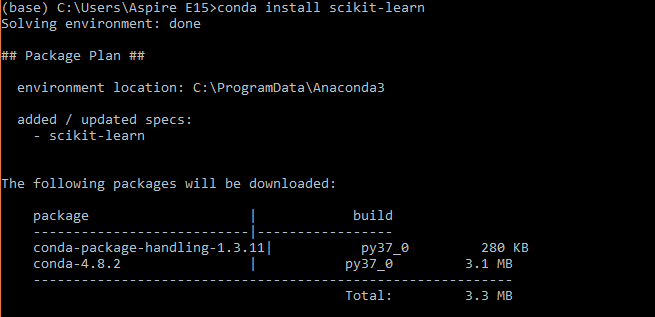
\includegraphics[width=4cm]{figures/1174074/1/Sckit-learn.png}
		\centering
		\caption{Instalasi Package Scikit Learn}
	\end{figure}
	\begin{figure}[H]
		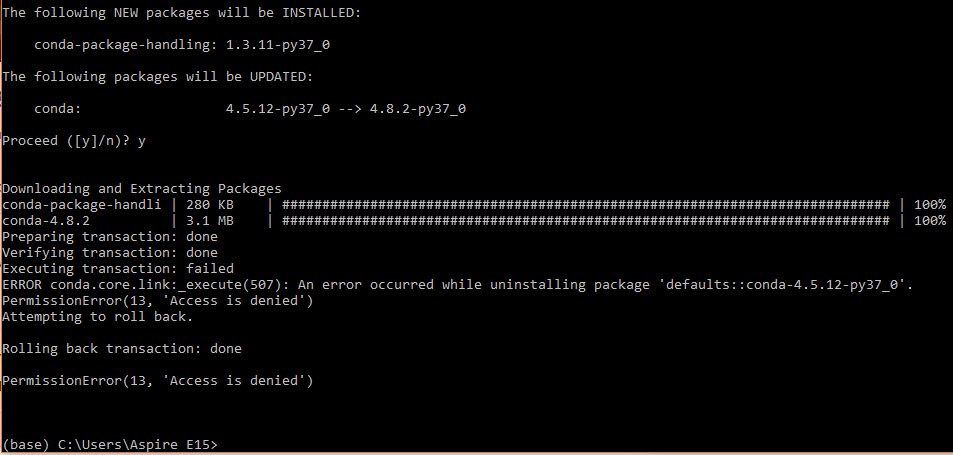
\includegraphics[width=4cm]{figures/1174074/1/Sckit-learn2.png}
		\centering
		\caption{Isi Variabel Explorer}
	\end{figure}
	\item Mencoba loading an example dataset
	\hfill\break
	\lstinputlisting[firstline=7, lastline=11]{src/1174074/1/1174074.py}
	\item Mencoba Learning dan predicting
	\hfill\break
	\lstinputlisting[firstline=12, lastline=22]{src/1174074/1/1174074.py}
	\item Mencoba Model Persistence
	\hfill\break
	\lstinputlisting[firstline=23, lastline=33]{src/1174074/1/1174074.py}
	\item Mencoba Conventions
	\hfill\break
	\lstinputlisting[firstline=34, lastline=46]{src/1174074/1/1174074.py}
\end{enumerate}
\subsection{Bukti Tidak Plagiat}
\begin{figure}[H]
	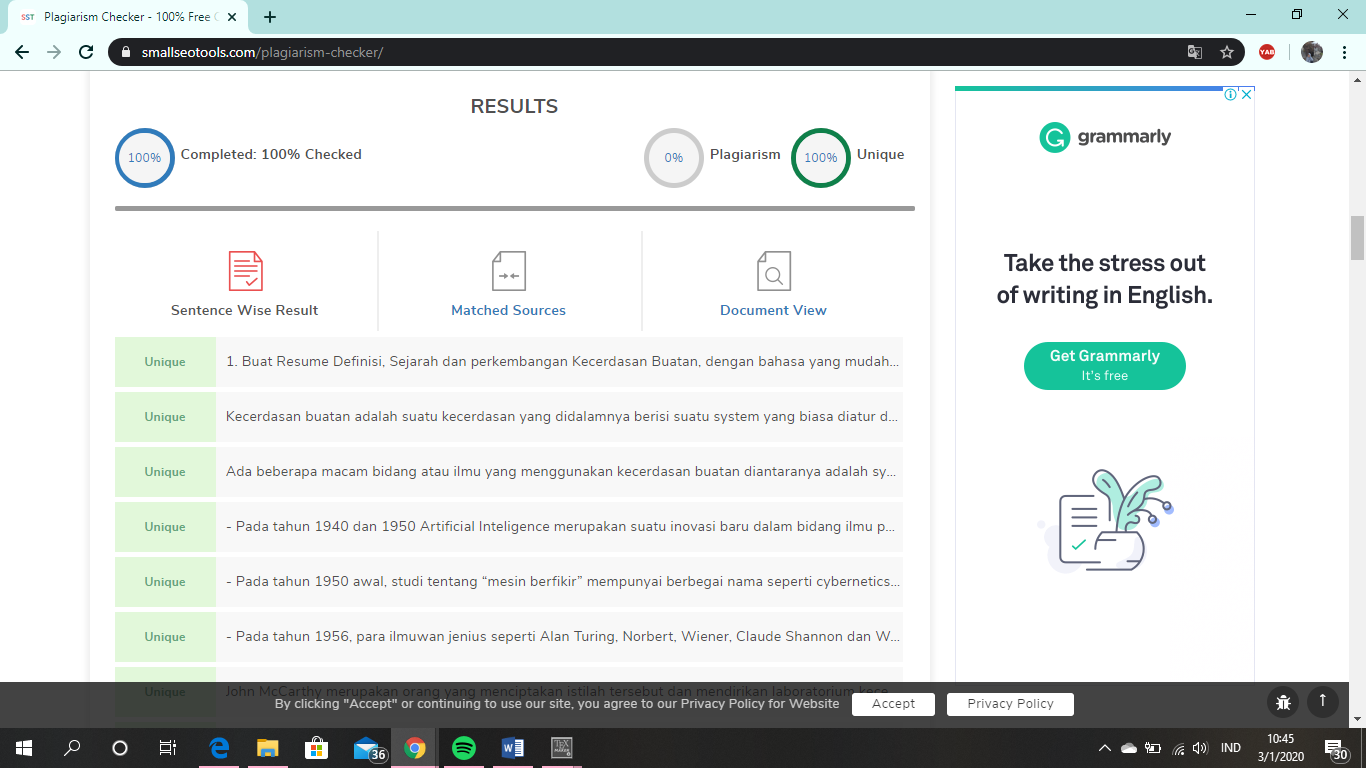
\includegraphics[width=4cm]{figures/1174074/1/plagiarisme.png}
	\centering
	\caption{Bukti Tidak Melakukan Plagiat}
\end{figure}